%Version 3 December 2023
% See section 11 of the User Manual for version history
%
%%%%%%%%%%%%%%%%%%%%%%%%%%%%%%%%%%%%%%%%%%%%%%%%%%%%%%%%%%%%%%%%%%%%%%
%%                                                                 %%
%% Please do not use \input{...} to include other tex files.       %%
%% Submit your LaTeX manuscript as one .tex document.              %%
%%                                                                 %%
%% All additional figures and files should be attached             %%
%% separately and not embedded in the \TeX\ document itself.       %%
%%                                                                 %%
%%%%%%%%%%%%%%%%%%%%%%%%%%%%%%%%%%%%%%%%%%%%%%%%%%%%%%%%%%%%%%%%%%%%%

%%\documentclass[referee,sn-basic]{sn-jnl}% referee option is meant for double line spacing

%%=======================================================%%
%% to print line numbers in the margin use lineno option %%
%%=======================================================%%

%%\documentclass[lineno,sn-basic]{sn-jnl}% Basic Springer Nature Reference Style/Chemistry Reference Style

%%======================================================%%
%% to compile with pdflatex/xelatex use pdflatex option %%
%%======================================================%%

%%\documentclass[pdflatex,sn-basic]{sn-jnl}% Basic Springer Nature Reference Style/Chemistry Reference Style


%%Note: the following reference styles support Namedate and Numbered referencing. By default the style follows the most common style. To switch between the options you can add or remove “Numbered” in the optional parenthesis. 
%%The option is available for: sn-basic.bst, sn-vancouver.bst, sn-chicago.bst%  
 
%%\documentclass[pdflatex,sn-nature]{sn-jnl}% Style for submissions to Nature Portfolio journals
%%\documentclass[pdflatex,sn-basic]{sn-jnl}% Basic Springer Nature Reference Style/Chemistry Reference Style
\documentclass[pdflatex,sn-mathphys-num]{sn-jnl}% Math and Physical Sciences Numbered Reference Style 
%%\documentclass[pdflatex,sn-mathphys-ay]{sn-jnl}% Math and Physical Sciences Author Year Reference Style
%%\documentclass[pdflatex,sn-aps]{sn-jnl}% American Physical Society (APS) Reference Style
%%\documentclass[pdflatex,sn-vancouver,Numbered]{sn-jnl}% Vancouver Reference Style
%%\documentclass[pdflatex,sn-apa]{sn-jnl}% APA Reference Style 
%%\documentclass[pdflatex,sn-chicago]{sn-jnl}% Chicago-based Humanities Reference Style

%%%% Standard Packages
%%<additional latex packages if required can be included here>

\usepackage{graphicx}%
\usepackage{multirow}%
\usepackage{amsmath,amssymb,amsfonts}%
\usepackage{amsthm}%
\usepackage{mathrsfs}%
\usepackage[title]{appendix}%
\usepackage{xcolor}%
\usepackage{textcomp}%
\usepackage{manyfoot}%
\usepackage{booktabs}%
\usepackage{algorithm}%
\usepackage{algorithmicx}%
\usepackage{algpseudocode}%
\usepackage{listings}%
\usepackage{xcolor} % TEMP - to delete later

% Custom packages
\usepackage{lineno}
\usepackage{comment}
\linenumbers
\usepackage{listings}%
\definecolor{codegreen}{rgb}{0,0.6,0}
\definecolor{codegray}{rgb}{0.5,0.5,0.5}
\definecolor{codepurple}{rgb}{0.58,0,0.82}
\definecolor{backcolour}{rgb}{0.95,0.95,0.92}
\lstdefinestyle{mystyle}{
    backgroundcolor=\color{backcolour},   
    commentstyle=\color{codegreen},
    keywordstyle=\color{magenta},
    numberstyle=\tiny\color{codegray},
    stringstyle=\color{codepurple},
    basicstyle=\ttfamily\footnotesize,
    breakatwhitespace=false,         
    breaklines=true,                 
    captionpos=b,                    
    keepspaces=true,                 
    numbers=left,                    
    numbersep=5pt,                  
    showspaces=false,                
    showstringspaces=false,
    showtabs=false,                  
    tabsize=2
}
\lstset{style=mystyle}

%%%%%=============================================================================%%%%
%%%%  Remarks: This template is provided to aid authors with the preparation
%%%%  of original research articles intended for submission to journals published 
%%%%  by Springer Nature. The guidance has been prepared in partnership with 
%%%%  production teams to conform to Springer Nature technical requirements. 
%%%%  Editorial and presentation requirements differ among journal portfolios and 
%%%%  research disciplines. You may find sections in this template are irrelevant 
%%%%  to your work and are empowered to omit any such section if allowed by the 
%%%%  journal you intend to submit to. The submission guidelines and policies 
%%%%  of the journal take precedence. A detailed User Manual is available in the 
%%%%  template package for technical guidance.
%%%%%=============================================================================%%%%

%%\unnumbered% uncomment this for unnumbered level heads

\begin{document}

\title[\hspace{14mm}\textbf{SUPPLEMENTARY MATERIAL} \newline Modularity maximization and community detection in complex networks through recursive and hierarchical annealing in the DWAVE Advantage quantum processing units]{\hspace{14mm}\textbf{SUPPLEMENTARY MATERIAL} \newline Modularity maximization and community detection in complex networks through recursive and hierarchical annealing in the DWAVE Advantage quantum processing units}

%%=============================================================%%
%% GivenName	-> \fnm{Joergen W.}
%% Particle	-> \spfx{van der} -> surname prefix
%% FamilyName	-> \sur{Ploeg}
%% Suffix	-> \sfx{IV}
%% \author*[1,2]{\fnm{Joergen W.} \spfx{van der} \sur{Ploeg} 
%%  \sfx{IV}}\email{iauthor@gmail.com} %%=============================================================%%

\author*[1]{\fnm{Joan} \sur{Falc\'o-Roget}}\email{j.roget@sanoscience.org, kzajac@agh.edu.pl}

\author[2,3]{\fnm{Kacper} \sur{Jurek}}
\equalcont{These authors contributed equally to this work.}

\author[1,2]{\fnm{Barbara} \sur{Wojtarowicz}}
\equalcont{These authors contributed equally to this work.}

\author[1,2]{\fnm{Karol} \sur{Capa{\l}a}}

\author*[1,2,3]{\fnm{Katarzyna} \sur{Rycerz}}

\affil[1]{\orgname{Sano - Centre for Computational Medicine}, \orgaddress{\street{Nawojki 11}, \city{Krakow}, \postcode{30-072}, \country{Poland}}}

\affil[2]{\orgdiv{Faculty of Computer Science}, \orgname{AGH University of Krakow}, \orgaddress{\street{Mickiewicza 30}, \city{Krak\'ow}, \postcode{30-059}, \country{Poland}}}

\affil[3]{\orgdiv{Quantum Computing Lab}, \orgname{Academic Computer Center Cyfronet AGH}, \orgaddress{\street{Nawojki 11}, \city{Krakow}, \postcode{30-950}, \country{Poland}}}

%%==================================%%
%% Sample for unstructured abstract %%
%%==================================%%

\abstract{In these supplements we provide detailed mathematical descriptions of the properties that the modularity function, matrix, and generalized versions have. These properties are necessary for the correct derivation of the function to optimize. We show how multiple scenarios fit within the same optimization framework, including an arbitrary resolution parameter and binary, weighted, and directed networks. Noteworthy, in the accompanying Python code, we included a Jupyter notebook where we numerically proof each one of the equations derived in this supplement. We also include the supplementary figures mentioned in the main text at the end.}

%%================================%%
%% Sample for structured abstract %%
%%================================%%

% \abstract{\textbf{Purpose:} The abstract serves both as a general introduction to the topic and as a brief, non-technical summary of the main results and their implications. The abstract must not include subheadings (unless expressly permitted in the journal's Instructions to Authors), equations or citations. As a guide the abstract should not exceed 200 words. Most journals do not set a hard limit however authors are advised to check the author instructions for the journal they are submitting to.
% 
% \textbf{Methods:} The abstract serves both as a general introduction to the topic and as a brief, non-technical summary of the main results and their implications. The abstract must not include subheadings (unless expressly permitted in the journal's Instructions to Authors), equations or citations. As a guide the abstract should not exceed 200 words. Most journals do not set a hard limit however authors are advised to check the author instructions for the journal they are submitting to.
% 
% \textbf{Results:} The abstract serves both as a general introduction to the topic and as a brief, non-technical summary of the main results and their implications. The abstract must not include subheadings (unless expressly permitted in the journal's Instructions to Authors), equations or citations. As a guide the abstract should not exceed 200 words. Most journals do not set a hard limit however authors are advised to check the author instructions for the journal they are submitting to.
% 
% \textbf{Conclusion:} The abstract serves both as a general introduction to the topic and as a brief, non-technical summary of the main results and their implications. The abstract must not include subheadings (unless expressly permitted in the journal's Instructions to Authors), equations or citations. As a guide the abstract should not exceed 200 words. Most journals do not set a hard limit however authors are advised to check the author instructions for the journal they are submitting to.}

\keywords{Quantum Annealing, Modularity Maximization, Community Detection, Complex Networks, Brain Connectivity}

%%\pacs[JEL Classification]{D8, H51}

%%\pacs[MSC Classification]{35A01, 65L10, 65L12, 65L20, 65L70}

\maketitle

\setcounter{figure}{0}
\renewcommand{\thefigure}{S\arabic{figure}}
\setcounter{equation}{0}
\renewcommand{\theequation}{S1.\arabic{equation}}
\setcounter{section}{0}
\renewcommand{\thesection}{S\arabic{section}}

\section{Weighted and undirected networks} \label{app:A}
For an undirected network, Newman's quality function for a given community structure consisting of only two modules is written as \cite{Wierzbinski2023}:
\begin{equation} \label{eq_A:ising}
    \begin{split}
        Q & = \sum_{c=1}^{2}\left[ \frac{L_c}{m} - \gamma \left(\frac{g_c}{2m}\right)^2\right] \\
          & = \frac{1}{2m} \sum_{ij\in G}\left( A_{ij} - \gamma \frac{g_i g_j}{2m} \right) \left(\frac{s_i s_j + 1}{2}\right)\\
          & = \frac{1}{4m} \sum_{ij\in G} B_{ij} s_i s_j + \frac{(1-\gamma)}{2},
    \end{split}
\end{equation} Quantum annealing (QA) works directly in binary variables $x_i=\{0,1\}$ instead of spin-like ones. We perform a simple transformation $s_i = 2x_i - 1$ for that. With this in mind, the complete quality function is as follows:
\begin{equation} \label{eq_A:QUBO}
    Q = \frac{1}{m}\sum_{ij\in G} B_{ij} x_i x_j - \frac{(1-\gamma)}{m}\sum_{i\in G} g_{i} x_i + 1-\gamma.
\end{equation}

Since QA minimizes a function up to a constant we can rewrite the function to optimize as follows:

\begin{equation} \label{eq_A:QUBO_optim}
    \begin{split}
        \Tilde{Q} & \doteq - m \left(Q - 1 + \gamma \right) \\
                  & = -\sum_{ij\in G} B_{ij} x_i x_j + (1-\gamma)\sum_{i\in G} g_{i} x_i \\
                  & = -\sum_{ij\in G} \left( A_{ij} - \gamma \frac{g_i g_j}{2m} \right) x_i x_j + (1-\gamma)\sum_{i\in G} g_{i} x_i,
    \end{split}
\end{equation} which can be optimized via QA to obtain high-quality divisions of a network into two communities \cite{Ushijima-Mwesigwa2017,Negre2020,Nembrini2022,Wierzbinski2023}. Thus, we base our method on the fact that QA works well in simple QUBO problems without one-hot encoding.

\subsection{Properties of the symmetric modularity matrix}
The sum of the elements in a single column (rows):
\begin{equation}\label{eq_A:sym_und_rows}
    \sum_{j \in G}B_{ij} = \sum_{j \in G}\left( A_{ij} - \gamma \frac{g_i g_j}{2m}\right) = (1 - \gamma)g_i.
\end{equation}
The sum of the elements in a single row (columns):
\begin{equation}\label{eq_A:sym_und_cols}
    \sum_{i \in G}B_{ij} = \sum_{i \in G}\left( A_{ij} - \gamma \frac{g_i g_j}{2m}\right) = (1 - \gamma)g_j.
\end{equation}
Given that the matrix is symmetric, $\forall i,j \in G$ the following also holds: $g_i=g_j$. Finally, the sum of all elements,
\begin{equation} \label{eq_A:sym_und_elements}
    \sum_{ij \in G}B_{ij} = 2m(1-\gamma).
\end{equation} With these, we can rewrite the modularity $Q$ using both Ising and binary variables (i.e., Eqs. \ref{eq_A:ising} and \ref{eq_A:QUBO}).

\subsection{Properties of the symmetric generalized modularity matrix}

\textit{The entire network forms a single community }($g=G$):

The generalized modularity matrix \textbf{B}\textsuperscript{g} can be simplified to
\begin{equation} \label{eq_A:gen_mod_full_G}
    \begin{split}
    B^{\text{g}}_{ij} & = B_{ij} - \delta_{ij}\sum_{k \in G} B_{ik} \\
                      & = B_{ij} - (1-\gamma)g_i\delta_{ij}, \\
    \end{split}
\end{equation} where the second equality follows from Eqs. \ref{eq_A:sym_und_rows}, \ref{eq_A:sym_und_cols} and, as stated in the main text, $\delta_{ij}$ is the Kronecker delta function. The following is thus straightforward, but for completeness, we explicitly sum the elements of rows and columns. The sum of the elements in a single column (rows):
\begin{equation}\label{eq_A:gen_sym_und_rows_full_g}
    \begin{split}
    \sum_{j \in G} B^{\text{g}}_{ij} & = \sum_{j \in G} \left[ B_{ij} - (1-\gamma)g_i\delta_{ij} \right ]\\
                                     & = (1-\gamma)g_i - (1-\gamma)g_i \sum_{j \in G} \delta_{ij} \\
                                     & = 0 \ \ \forall \gamma,
    \end{split}
\end{equation} where the third equality stems from $\sum_{i \in G} \delta_{ij}=1$. The sum of the elements in a single row (columns): 
\begin{equation}\label{eq_A:gen_sym_und_cols_full_g}
    \begin{split}
    \sum_{i \in G} B^{\text{g}}_{ij} & = \sum_{i \in G} \left[ B_{ij} - (1-\gamma)g_i\delta_{ij} \right ] \\
                                     & = (1-\gamma)g_j - (1-\gamma)g_j \sum_{i \in G} \delta_{ij} \\
                                     & = 0 \ \ \forall \gamma,
    \end{split}
\end{equation} where, once again, the third equality is true given that $g=G$. Contrary to the modularity matrix \textbf{B}, the sum of all elements of the generalized modularity matrix \textbf{B}\textsuperscript{g} is equal to zero, that is,  $\forall \gamma$,
\begin{equation} \label{eq_A:gen_sym_und_elements_full_g}
    \sum_{ij \in G}B^{\text{g}}_{ij}=0.
\end{equation} Noteworthy, the two matrices are identical if the resolution parameter is equal to 1 \cite{Newman2006}.

\textit{The entire network has already been divided into an arbitrary number of communities and we wish to further subdivide one of them} ($g \subset G$):

The sum of the elements in a single column (rows):
\begin{equation}\label{eq_A:gen_sym_und_cols_g}
    \begin{split}
    \sum_{j \in g} B^{\text{g}}_{ij} & = \sum_{j \in g} \left[ B_{ij} - \delta_{ij}\sum_{k \in g} B_{ik} \right ] \\
    & = \sum_{j \in g} \left[ A_{ij} - \gamma \frac{g_i g_j}{2m} - \delta_{ij}\sum_{k \in g} \left( A_{ik} - \gamma \frac{g_i g_k}{2m}\right) \right ] \\
    & = \sum_{j \in g} A_{ij} - \frac{\gamma g_i}{2m} \sum_{j \in g}g_j - \sum_{j \in g} \delta_{ij}\sum_{k \in g} A_{ik} + \frac{\gamma g_i}{2m}\sum_{j \in g} \delta_{ij} \sum_{k \in g} g_k \\
    &= \sum_{j \in g} A_{ij} - \sum_{j \in g} \delta_{ij}\sum_{k \in g} A_{ik} - \frac{\gamma g_i}{2m} \left[ \sum_{j \in g}g_j - \sum_{j \in g} \delta_{ij} \sum_{k \in g} g_k \right] \\
    &= \sum_{j \in g} A_{ij} - \sum_{k \in g} A_{ik} - \frac{\gamma g_i}{2m} \left[ \sum_{j \in g}g_j - \sum_{k \in g} g_k \right] \\
    & = 0 \ \ \forall \gamma,
    \end{split}
\end{equation} where we have used $\sum_{j \in g}\delta_{ij}=1$. A similar derivation could be done for the sum of the elements in a single column (rows); however, we can use make use of the fact that the modularity matrix is symmetric for this case. That is,
\begin{equation}\label{eq_A:gen_sym_und_rows_g}
    \sum_{i \in g} B^{\text{g}}_{ij} = \sum_{i \in g} B^{\text{g}}_{ji} = 0 \ \ \forall \gamma.
\end{equation} Therefore, as opposed to the sum of the elements of the modularity matrix, the sum of the elements in $g$ of the generalized modularity matrix add up to zero for an arbitrary resolution parameter; that is, $\forall \gamma$,
\begin{equation} \label{eq_A:gen_sym_und_elements_g}
    \sum_{ij \in g}B^{\text{g}}_{ij}=0.
\end{equation} 

\begin{comment}
\color{red} WHAT FOLLOWS IS NOT REALLY NEEDED BUT IT WAS USEFUL FOR MY BETTER UNDERSTANDING. WE CAN JUST DROP IT WHEN THE TIME COMES.

To make the expression more tractable and at the same gain intuition, we shall define four quantities that, in turn, will prove useful.
\begin{itemize}
    \item The \textit{within-community degree} quantifies the number of weighted connections a given node has with neighbors inside the community.
    \begin{equation} \label{eq_A:within_deg_und}
        \begin{split}
            g_{i}^{\text{g}} & \doteq \sum_{k \in g} \delta_{ik} \sum_{j \in g} A_{kj} \\
            g_{j}^{\text{g}} & \doteq \sum_{k \in g} \delta_{kj} \sum_{i \in g} A_{ik}, \\
        \end{split}
    \end{equation} where Kronecker delta is needed to ensure that only nodes belonging to the community are considered.
    \item The \textit{wihtin-community edges} measures the total number of edges between nodes in the community.    
    \begin{equation} \label{eq_A:within_edge_und}
        \begin{split}
        m^{\text{g}} & \doteq \frac{1}{2} \sum_{i \in g} g_{i}^{\text{g}} \\
                       & = \frac{1}{2} \sum_{i \in g}  \sum_{k \in g} \delta_{kj} \sum_{j \in g} A_{kj} \\
                       & = \frac{1}{2} \sum_{i \in g} \sum_{j \in g} A_{ij}. \\
        \end{split}
    \end{equation}
    \item The \textit{between-community degree} quantifies the number of weighted connections a given node has with neighbors outside the community.
    \begin{equation} \label{eq_A:between_deg_und}
        \begin{split}
            g_{i}^{\text{\~g}} & \doteq \sum_{k \in g} \delta_{ik} \sum_{j \notin g} A_{kj} \\
            g_{j}^{\text{\~g}} & \doteq \sum_{k \in g} \delta_{kj} \sum_{i \notin g} A_{ik}, \\
        \end{split}
    \end{equation}
    \item The \textit{between-community edges} measures the total number of edges that nodes inside the community have with nodes outside of it.
    \begin{equation} \label{eq_A:between_edge_und}
        \begin{split}
        m^{\text{\~g}} & \doteq \sum_{i \in g} g_{i}^{\text{\~g}} \\
                       & = \sum_{i \in g}  \sum_{k \in g} \delta_{ik} \sum_{j \notin g} A_{kj}  \\
                       & = \sum_{i \in g} \sum_{j \notin g} A_{ij}. \\
        \end{split}
    \end{equation} Intuitively, the last term is the sum of the \textit{off-block} diagonal elements of the adjacency matrix when sorted by communities. Importantly, the four quantities defined above behave as expected when the network contains a single community. That is, $g_{i}^{\text{g}} \to g_i$, $m^{\text{g}} \to m$, $g_{i}^{\text{\~g}} \to 0$, and $m^{\text{\~g}} \to 0$. It could prove insightful to think of community detection algorithms as processes trying to find the set of non-overlapping (in principle) communities $C=\{g \ | \ \forall g \subset G\}$ that jointly maximize $\mathbb{E}_g\left[m^{\text{g}}\right]$ and minimize $\mathbb{E}_g\left[m^{\text{\~g}}\right]$. Furthermore, the weighted degree can be effectively decomposed as a sum of the \textit{within-community} and \textit{betwee-community} degrees.
    \begin{equation} \label{eq_A:sum_degrees_gen}
        \begin{split}
            g_{i}^{\text{g}}+g_{i}^{\text{\~g}} &= \sum_{k \in g} \delta_{ik} \sum_{j \in g} A_{kj} + \sum_{k \in g} \delta_{ik} \sum_{j \notin g} A_{kj} \\
            &= \sum_{k \in g} \delta_{ik} \left[ \sum_{j \in g} A_{kj} + \sum_{j \notin g} A_{kj}\right] \\
            &= \sum_{k \in g} \delta_{ik} \sum_{j \in g} A_{kj} \\
            &= \sum_{k \in g} \delta_{ik} g_k \\
            &= g_i \ \ \ q.e.d.
        \end{split}
    \end{equation} Noteworthy, the same shan't be naively assumed for the number of edges. 
\end{itemize}
\color{black}
\end{comment}

\setcounter{equation}{0}
\renewcommand{\theequation}{S2.\arabic{equation}}
\section{Weighted and directed networks} \label{app:B}
For directed networks, the quality function is slightly different but the procedure is similar to the one outlined before.
\begin{equation} \label{eq_B:ising_dir}
    \begin{split}
        Q & = \sum_{c=1}^{2}\left[ \frac{L_c}{m} - \gamma \left(\frac{g_c^{in}g_c^{out}}{m^2}\right)\right] \\
          & = \frac{1}{m} \sum_{ij\in G}\left( A_{ij} - \gamma \frac{g_i^{in} g_j^{out}}{m} \right) \left(\frac{s_i s_j + 1}{2}\right)\\
          & = \frac{1}{2m} \sum_{ij\in G} B_{ij}^{d} s_i s_j + \frac{(1-\gamma)}{2},
    \end{split}
\end{equation} where $B_{ij}^d = A_{ij} - \gamma \frac{g_i^{in} g_j^{out}}{m}$ is the now the \textit{directed} modularity matrix, $m=\sum_{ij}A_{ij}$ is the total edge-weight, $g_i^{in}=\sum_j A_{ij}$ is the node weighted in-degree, $g_j^{out}=\sum_i A_{ij}$ is the node weighted out-degree, and $s_i = \{-1,1\} \ \forall i \in G$ are spin-like variables. Once again, we apply the same transformation $s_i=2x_i-1$ to obtain the quality function in terms of binary variables.

\begin{equation} \label{eq_B:QUBO_dir}
    Q = \frac{2}{m}\sum_{ij\in G} B_{ij}^d x_i x_j - \frac{(1-\gamma)}{m}\left[\sum_{i\in G} g_{i}^{in} x_i + \sum_{j\in G} g_{j}^{out} x_j\right] + 1-\gamma.
\end{equation}

Once again, we can optimize the previous function up to a constant. Then, we proceed in an identical manner:

\begin{equation} \label{eq_B:QUBO_dir_optim}
    \begin{split}
        \Tilde{Q} & \doteq - \frac{m}{2} \left(Q - 1 + \gamma \right) \\
                  & = -\sum_{ij\in G} B_{ij}^d x_i x_j + \frac{(1-\gamma)}{2}\left[\sum_{i\in G} g_{i}^{in} x_i + \sum_{j\in G} g_{j}^{out} x_j \right]\\
                  & = -\sum_{ij\in G} \left( A_{ij} - \gamma \frac{g_i^{in} g_j^{out}}{m} \right) x_i x_j + \frac{(1-\gamma)}{2}\left[\sum_{i\in G} g_{i}^{in} x_i + \sum_{j\in G} g_{j}^{out} x_j \right].
    \end{split}
\end{equation} which can be optimized via QA to obtain high-quality divisions of a directed network into two communities. Noteworthy, the undirected and directed cases are equivalent only if the resolution is equal to 1. 

\subsection{Properties of the asymmetric modularity matrix}
The sum of the elements in a single column (rows):
\begin{equation}\label{eq_B:dir_rows}
    \sum_{j \in G}B_{ij}^d = \sum_{j \in G}\left( A_{ij} - \gamma \frac{g_{i}^{in} g_{j}^{out}}{m}\right) = (1 - \gamma)g_i^{in}.
\end{equation}
The sum of the elements in a single row (columns):
\begin{equation}\label{eq_B:dir_cols}
    \sum_{i \in G}B_{ij}^d = \sum_{i \in G}\left( A_{ij} - \gamma \frac{g_{i}^{in} g_{j}^{out}}{m}\right) = (1 - \gamma)g_j^{out}.
\end{equation}
Finally, the sum of all elements,
\begin{equation} \label{eq_B:dir_elements}
    \sum_{ij \in G}B_{ij}^d = m(1-\gamma).
\end{equation} With these, we can rewrite the modularity $Q$ using both Ising and binary variables (i.e., Eqs. \ref{eq_B:ising_dir} and \ref{eq_B:QUBO_dir}).

\subsection{Properties of the asymmetric generalized modularity matrix}

\textit{The entire network forms a single community }($g=G$):

The directed generalized modularity matrix \textbf{B}\textsuperscript{d,g} can be simplified to
\begin{equation} \label{eq_B:dire_gen_mod_full_G}
    \begin{split}
    B^{d,\text{g}}_{ij} & = B_{ij}^d - \delta_{ij}\sum_{k \in G} B_{ik}^d \\
                      & = B_{ij}^d - (1-\gamma)g_{i}^{in}\delta_{ij}, \\
    \end{split}
\end{equation} where the second equality follows from Eqs. \ref{eq_B:dir_rows}, \ref{eq_B:dir_cols} and, as stated in the main text, $\delta_{ij}$ is the Kronecker delta function. The following is thus straightforward, but for completeness, we explicitly sum the elements of rows and columns. The sum of the elements in a single column (rows):
\begin{equation}\label{eq_B:gen_dir_rows_full_g}
    \begin{split}
    \sum_{j \in G} B^{d,\text{g}}_{ij} & = \sum_{j \in G} \left[ B_{ij}^d - (1-\gamma)g_{i}^{in}\delta_{ij} \right ]\\
                                     & = (1 - \gamma)g_i^{in} - (1 - \gamma)g_i^{in} \sum_{j \in G} \delta_{ij} \\
                                     & = 0 \ \ \forall \gamma,
    \end{split}
\end{equation} where the third equality stems from $\sum_{i \in G} \delta_{ij}=1$. The sum of the elements in a single row (columns): 
\begin{equation}\label{eq_B:gen_dir_cols_full_g}
    \begin{split}
    \sum_{i \in G} B^{d,\text{g}}_{ij} & = \sum_{i \in G} \left[ B_{ij}^d - (1-\gamma)g_{i}^{in}\delta_{ij} \right ] \\
                                     & = (1-\gamma)g_j^{out} - (1-\gamma) \sum_{i \in G} g_i^{in}\delta_{ij} \\
                                     & = (1-\gamma)(g_j^{out}-g_j^{in}) \ \ \forall \gamma.
    \end{split}
\end{equation} Contrary to the directed modularity matrix \textbf{B}, the sum of all elements of the directed generalized modularity matrix \textbf{B}\textsuperscript{d,g} is equal to zero, that is,  $\forall \gamma$,
\begin{equation} \label{eq_B:gen_dir_elements_full_g}
    \sum_{ij \in G}B^{\text{g}}_{ij}=0.
\end{equation} This is due to the fact that summing the in- and out-degrees is equivalent. Noteworthy, the two matrices are identical if the resolution parameter is equal to 1 \cite{Leicht2008}.

\textit{The entire network has already been divided into an arbitrary number of communities and we wish to further subdivide one of them} ($g \subset G$):

The sum of the elements in a single column (rows):
\begin{equation}\label{eq_B:gen_dir_cols_g}
    \begin{split}
    \sum_{j \in g} B^{d,\text{g}}_{ij} & = \sum_{j \in g} \left[ B^{d}_{ij} - \delta_{ij}\sum_{k \in g} B^{d}_{ik} \right ] \\
    & = \sum_{j \in g} \left[ A_{ij} - \gamma \frac{g^{in}_i g^{out}_j}{2m} - \delta_{ij}\sum_{k \in g} \left( A_{ik} - \gamma \frac{g^{in}_i g^{out}_k}{2m}\right) \right ] \\
    & = \sum_{j \in g} A_{ij} - \frac{\gamma g^{in}_i}{2m} \sum_{j \in g}g^{out}_j - \sum_{j \in g} \delta_{ij}\sum_{k \in g} A_{ik} + \frac{\gamma g^{in}_i}{2m}\sum_{j \in g} \delta_{ij} \sum_{k \in g} g^{out}_k \\
    &= \sum_{j \in g} A_{ij} - \sum_{j \in g} \delta_{ij}\sum_{k \in g} A_{ik} - \frac{\gamma g^{in}_i}{2m} \left[ \sum_{j \in g}g^{out}_j - \sum_{j \in g} \delta_{ij} \sum_{k \in g} g^{out}_k \right] \\
    &= \sum_{j \in g} A_{ij} - \sum_{k \in g} A_{ik} - \frac{\gamma g^{in}_i}{2m} \left[ \sum_{j \in g}g^{out}_j - \sum_{k \in g} g^{out}_k \right] \\
    & = 0 \ \ \forall \gamma,
    \end{split}
\end{equation}

Contrary to the symmetric case, the sum of the elements in a single rows (columns) is different than zero. To show this, we proceed similarly as above.
\begin{equation}\label{eq_B:gen_dir_rows_g}
    \begin{split}
    \sum_{i \in g} B^{d,\text{g}}_{ij} & = \sum_{j \in g} \left[ B^{d}_{ij} - \delta_{ij}\sum_{k \in g} B^{d}_{ik} \right ] \\
    & = \sum_{i \in g} B^{d}_{ij} - \left( \sum_{i \in g} \delta_{ij}\sum_{k \in g} B^{d}_{ik} \right ) \\
    & = \sum_{i \in g} B^{d}_{ij} - \sum_{k \in g} B^{d}_{jk}\\
    & = \sum_{i \in g} \left ( B^{d}_{ij} - B^{d}_{ji} \right ) \ \ \forall \gamma.
    \end{split}
\end{equation} In general, the above results are different zero given that the matrix is not symmetric (i.e., $B^{d}_{ij} \neq B^{d}_{ji}$). Straightforwardly, the sum of the elements in $g$ of the directed generalized modularity matrix also adds up to zero.
\begin{equation} \label{eq_B:gen_dir_elements_g}
    \sum_{ij \in g}B^{d,\text{g}}_{ij}=0.
\end{equation}

\subsection{Computation of the \textit{k}-th element of the process without symmetrizing the network}
Proceeding similarly to in the undirected case, The modularity of an undirected network of $|C^{k-1}|$ different communities can be decomposed as 
$$ Q(C^{k-1}) = \sum_{c \in \Tilde{C}^{k-2}} \left[ \frac{L_c}{m} - \gamma \left(\frac{g^{in}_c g^{out}_c}{m^2}\right)\right] + \frac{L_k}{m} - \gamma \left(\frac{g^{in}_k g^{out}_k}{m^2}\right) $$ where $\Tilde{C}^{k-2} \cup k = C^{k-1}$. Then, the modularity index of the same network after splitting the $k$-th community in two can also be decomposed as
$$ Q(C^{k}) = \sum_{c \in \Tilde{C}^{k-2}} \left[ \frac{L_c}{m} - \gamma \left(\frac{g^{in}_c g^{out}_c}{m^2}\right)\right] + \sum_{r=1}^{2} \left[ \frac{L_{k_{r}}}{m} - \gamma \left(\frac{g^{in}_{k_{r}} g^{out}_{k_{r}}}{m^2}\right) \right]$$ where $k_1 \cup k_2 = k$. Subtracting both expressions and using Eq. \ref{eq_B:ising_dir} we obtain a compact expression for the elements of $\mathcal{P}$ in terms of the directed modularity matrix,
\begin{equation} \label{eq_B:pk_dir}
    \begin{split}
        p_k &= \frac{-2}{m} \sum_{ij \in k} \left( B_{ij}^ds_i s_j - B^d_{ij}\right) - \frac{1-\gamma}{2} \\
        &= \frac{-2}{m} \sum_{ij \in k} \left( B^d_{ij} - \delta_{ij} \sum_{r\in k} B^d_{ir}\right)s_i s_j = \frac{-2}{m} \sum_{ij \in k} B_{ij}^{d,\text{k}} s_i s_j \\
        &= \frac{-2}{m} \left[ 4 \sum_{ij \in k} B_{ij}^{d,\text{k}} x_i x_j -2 \sum_{ij \in k} B_{ij}^{d,\text{k}} x_i + -2 \sum_{ij \in k} B_{ij}^{d,\text{k}} x_j + \sum_{ij \in k} B_{ij}^{d,\text{k}} \right]\\
        &= \frac{-8}{m} \left[ \sum_{ij \in k} B_{ij}^{d,\text{k}} x_i x_j  - \frac{1}{2} \sum_{j\in k} x_j \sum_{i\in k} \left(B_{ij}^d - B_{ji}^d \right)\right],
    \end{split}
\end{equation} where we have arbitrarily dropped the constant term $\frac{1-\gamma}{2}$, $\delta_{ij}$ is the Kronecker delta function, we used $s_i^2=1$, and 
\begin{equation} \label{eq_B:dir_gen_mod_matrix}
    B_{ij}^{d,\text{k}} = B_{ij}^d - \delta_{ij} \sum_{r\in k} B_{ir}^d \ \ \forall i,j \in k,
\end{equation}is the directed generalized modularity matrix \textbf{B}\textsuperscript{$d$,k} for the $k$-th community \cite{Newman2006}. In the second row, we have applied a linear mapping from the Ising variables to a set of binary ones $s_i=2x_i-1$ to obtain the QUBO formulation. The last row follows from some of the properties of the generalized modularity matrix outlined in the previous section in the Supplements.

Finally, for $k=0$, $$p_0 = -4 \left[ \frac{2}{m} \sum_{ij\in G} B_{ij}^d x_i x_j - \frac{2(1-\gamma)}{m}\sum_{i \in G} g^{in}_i x_i - \frac{1}{2m} \sum_{i\in k} x_i \left(B_{ij}^d - B_{ji}^d \right)\right],$$ which does not resemble Eqs. \ref{eq_B:QUBO_dir} or \ref{eq_B:QUBO_dir_optim}.

\clearpage
\section*{Supplementary figures}

\begin{figure}[h]
    \centering
    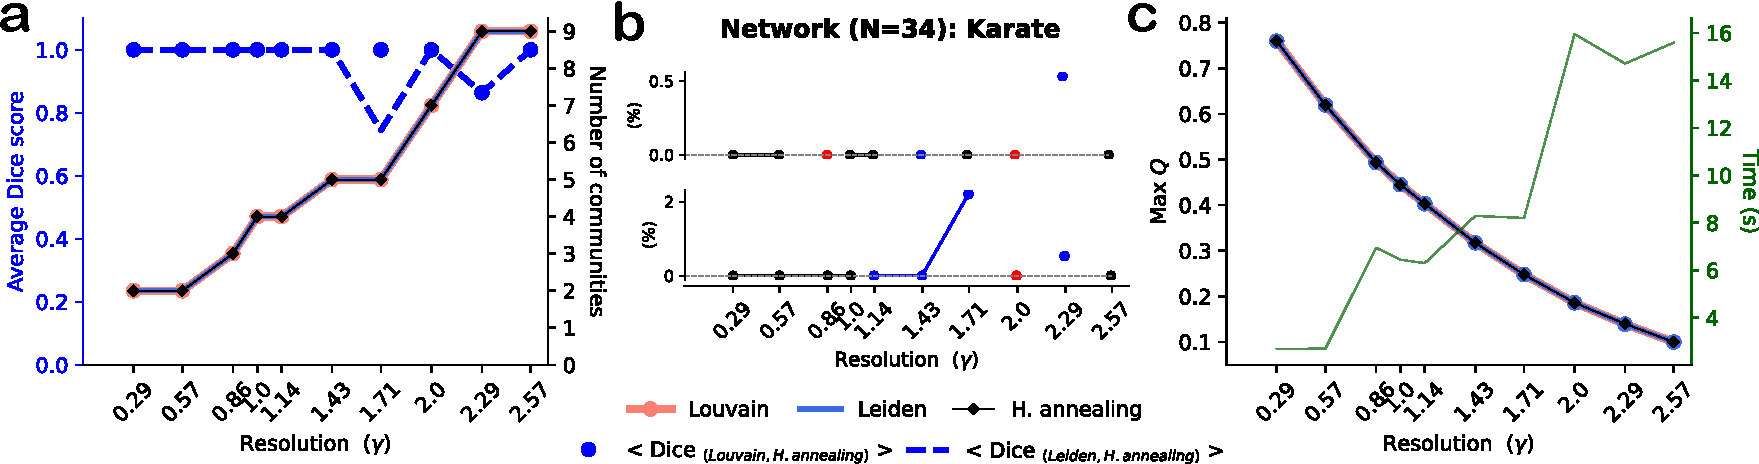
\includegraphics[width=1\linewidth]{Figures/FigS1.pdf}
    \caption{\textbf{Hierarchical annealing in the Karate Club network for different resolution parameters.} \textbf{a} Measure of the average overlap between the communities found by the Louvain and Hierarchical annealing algorithms (left axis, blue) and the number of communities (right axis, salmon and black) as a function of the resolution parameter $\gamma$. \textbf{b} Relative increase of the Hierarchical annealing measured w.r.t. the Louvain (top) and Leiden (bottom) solutions in \textbf{a}. Black, blue, and red symbols depict equal, better, and worse performance of the quantum method respectively. \textbf{c} Maximum modularity per resolution value (left axis, same legend as in \textbf{a}) and the total computing time per solution (right axis, green).}
    \label{fig:resolution_karate}
\end{figure}

\begin{figure}[h]
    \centering
    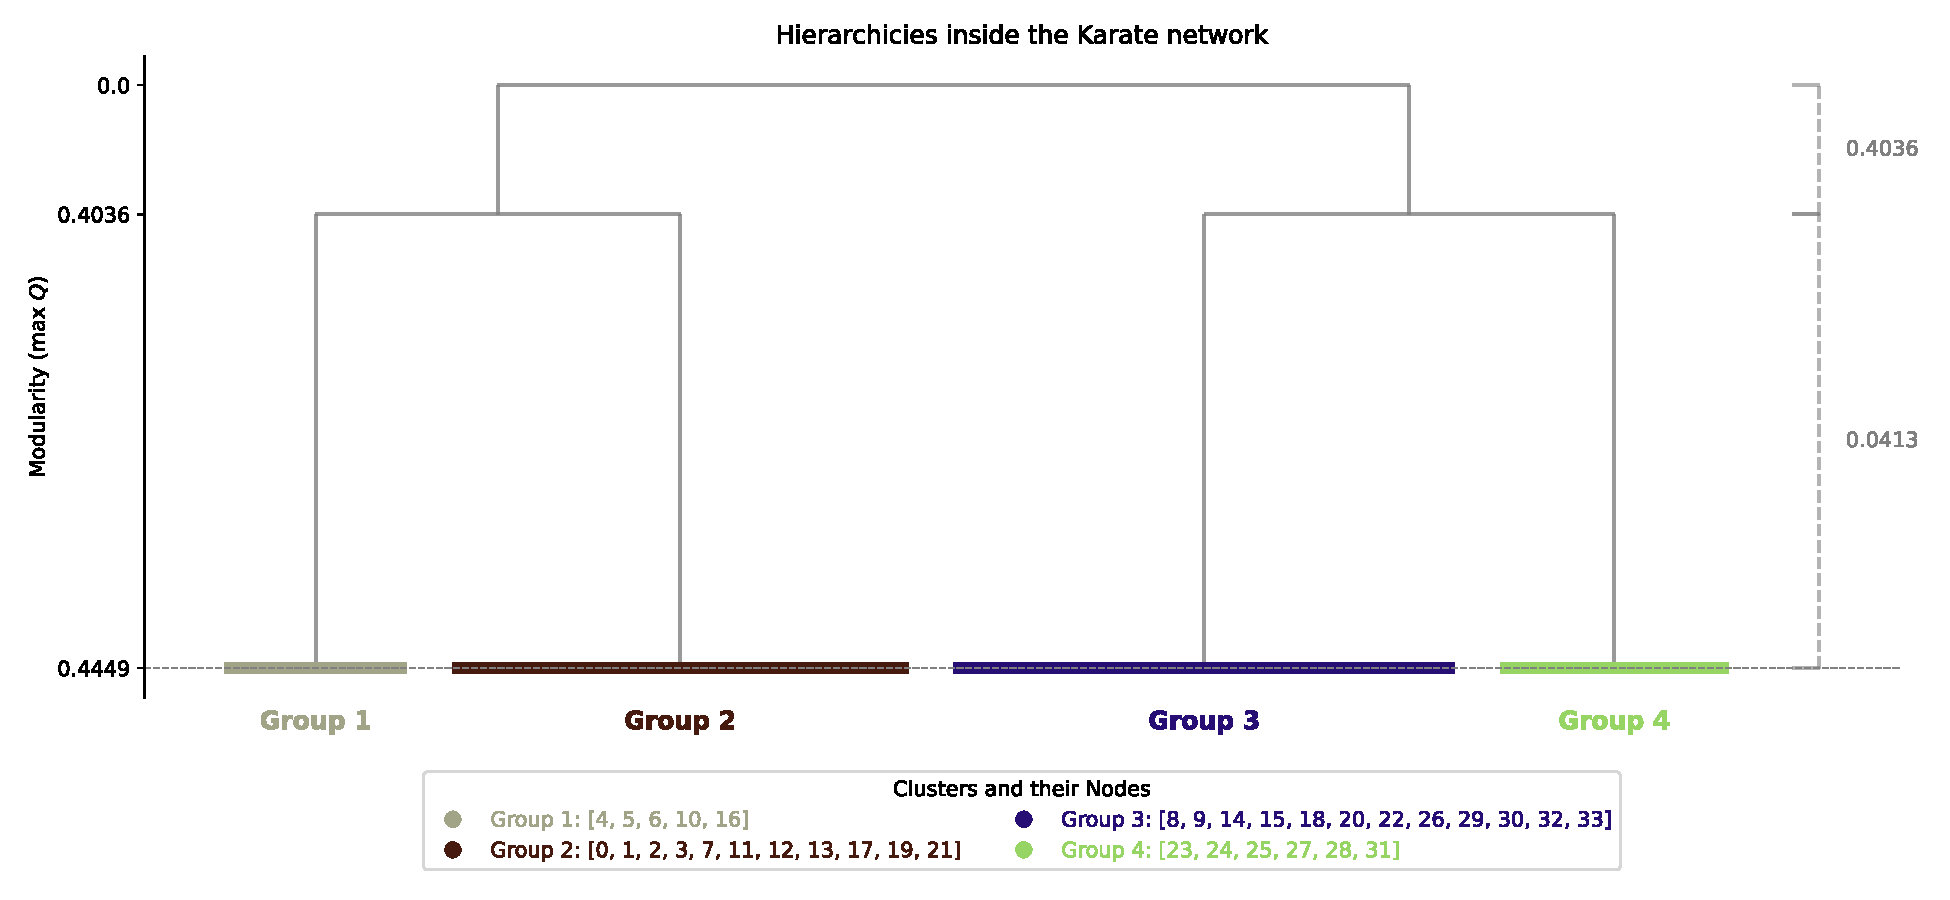
\includegraphics[width=1\linewidth]{Figures/FigS2.pdf}
    \caption{\textbf{Dendrogram of the Karate network \cite{zachary1977information}.} Hierarchical structure found by the H. annealing algorithm. The hierarchy corresponds to the one unraveled after maximizing the modularity of the network as described in the main text; that is, {\tt num\_runs = 50} and {\tt resolution = 1}. The left axis shows the modularity at each step of the process, while the right axis displays the corresponding increments. The bottom-most row represents the final output of the H. annealing algorithm.}
    \label{fig:dendro_karate}
\end{figure}

\begin{figure}[h]
    \centering
    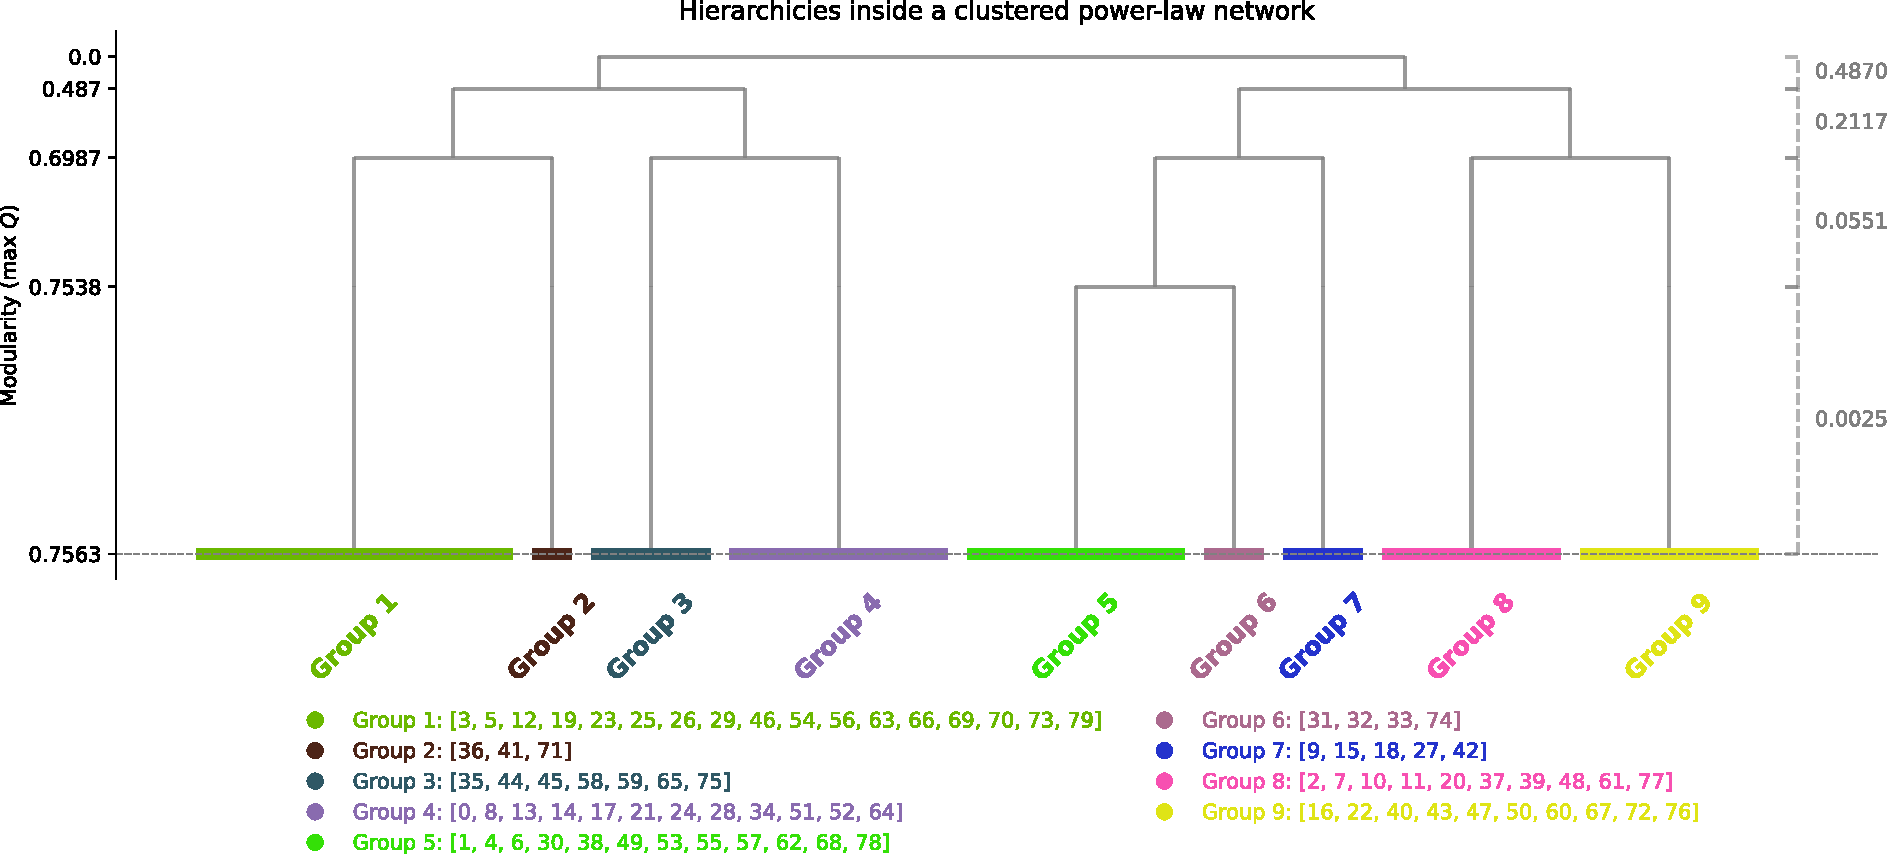
\includegraphics[width=1\linewidth]{Figures/FigS3.pdf}
    \caption{\textbf{Dendrogram of a clustered power-law network \cite{Holme2002} of N=80 nodes.} Hierarchical structure found by the H. annealing algorithm. The hierarchy corresponds to the one unraveled after maximizing the modularity of the network as described in the main text; that is, {\tt num\_runs = 10} and {\tt resolution = 1}. Both the Louvain and Leiden algorithms returned a maximum modularity of $Q=0.7563$. The left axis shows the modularity at each step of the process, while the right axis displays the corresponding increments. The bottom-most row represents the final output of the H. annealing algorithm.}
    \label{fig:dendro_pw}
\end{figure}

\begin{figure}[h]
    \centering
    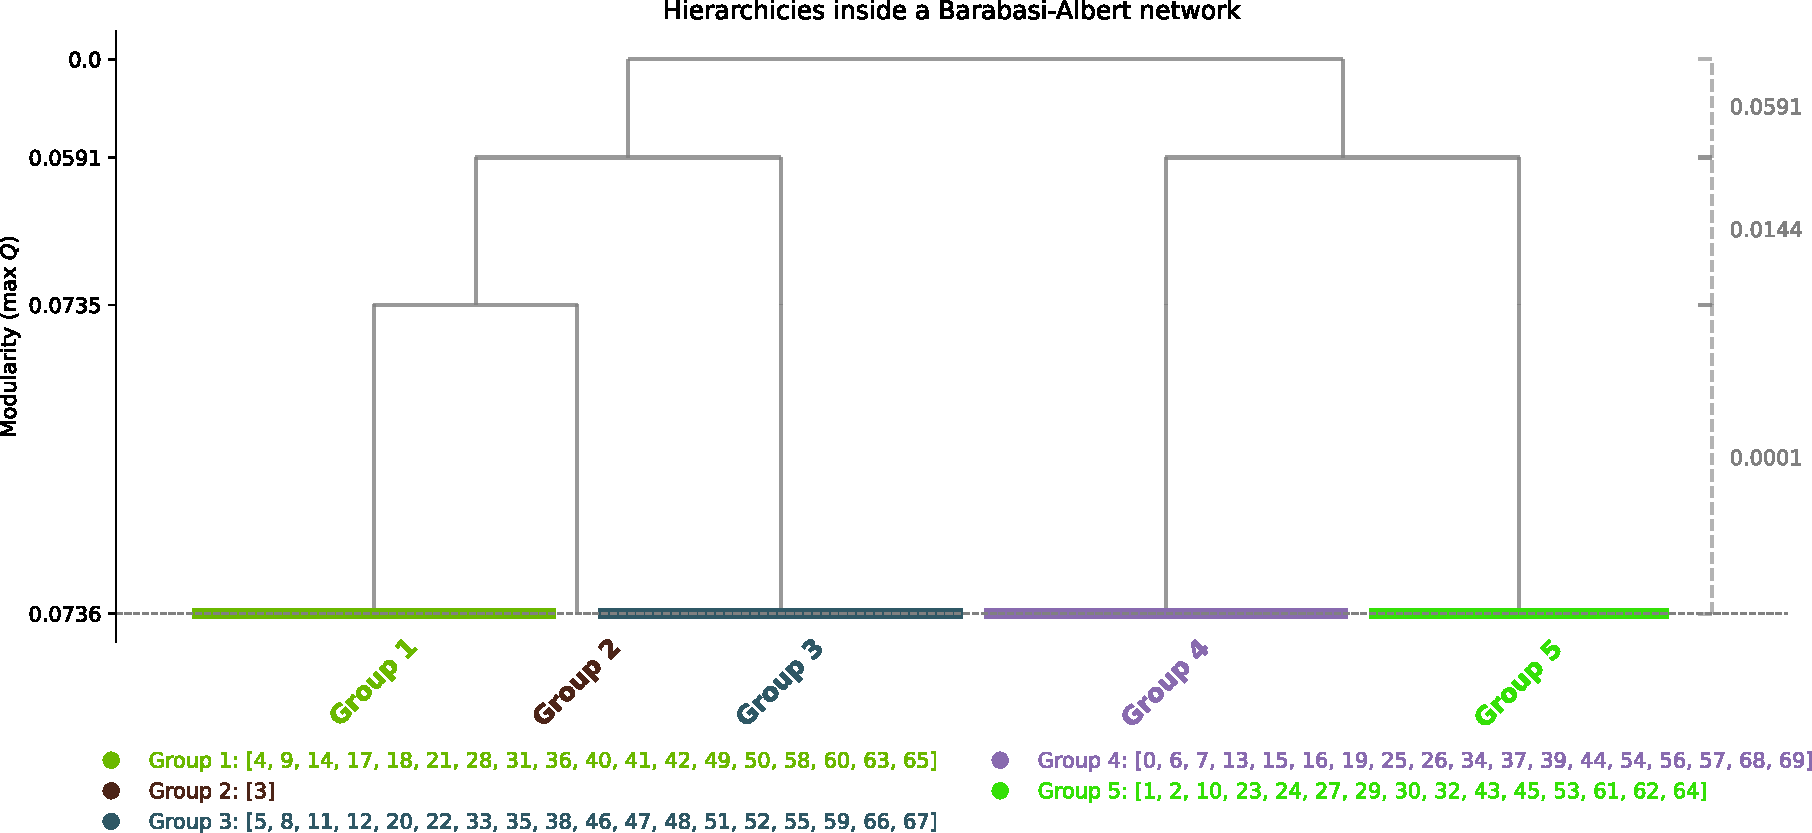
\includegraphics[width=1\linewidth]{Figures/FigS4.pdf}
    \caption{\textbf{Dendrogram of a Barabasi-Albert network \cite{Barabasi1999} of N=70 nodes.} Hierarchical structure found by the H. annealing algorithm. The hierarchy corresponds to the one unraveled after maximizing the modularity of the network as described in the main text; that is, {\tt num\_runs = 20} and {\tt resolution = 1}. The Louvain and Leiden algorithms returned maximum modularities of $Q=0.0760$ and $Q=0.0698$ respectively. The left axis shows the modularity at each step of the process, while the right axis displays the corresponding increments. The bottom-most row represents the final output of the H. annealing algorithm.}
    \label{fig:dendro_ba}
\end{figure}

\begin{figure}[h]
    \centering
    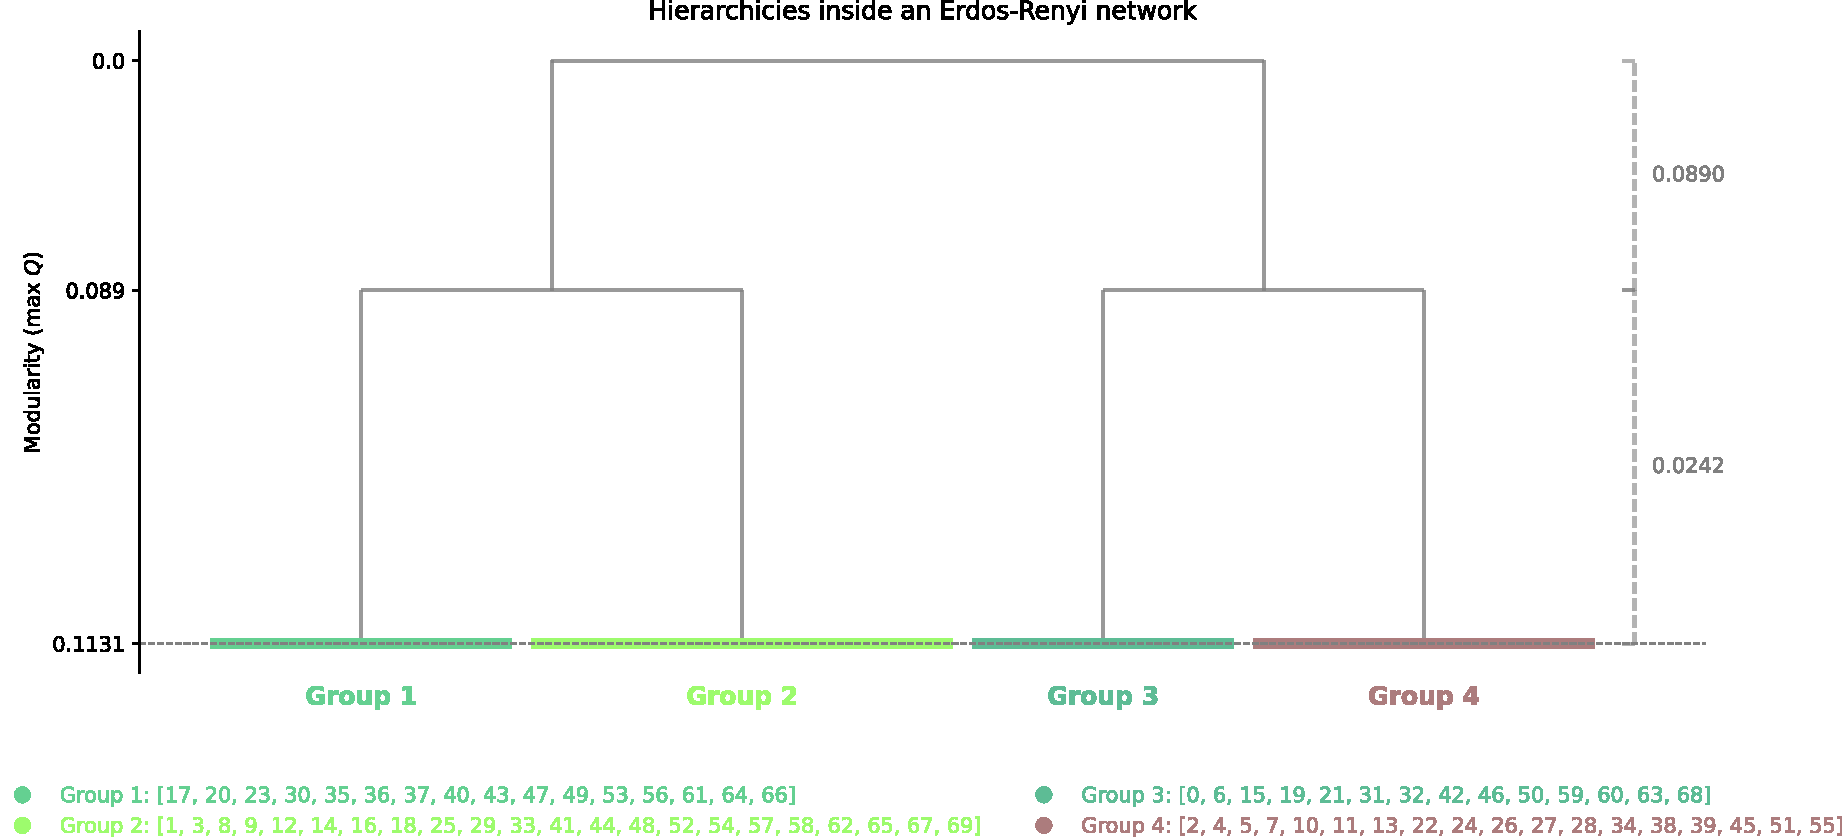
\includegraphics[width=1\linewidth]{Figures/FigS5.pdf}
    \caption{\textbf{Dendrogram of an Erdos-Renyi network \cite{erdds1959random} of N=70 nodes.} Hierarchical structure found by the H. annealing algorithm. The hierarchy corresponds to the one unraveled after maximizing the modularity of the network as described in the main text; that is, {\tt num\_runs = 50} and {\tt resolution = 1}. The Louvain and Leiden algorithms returned maximum modularities of $Q=0.1189$ and $Q=0.1021$ respectively. The left axis shows the modularity at each step of the process, while the right axis displays the corresponding increments. The bottom-most row represents the final output of the H. annealing algorithm.}
    \label{fig:dendro_er}
\end{figure}

\begin{figure}[h]
    \centering
    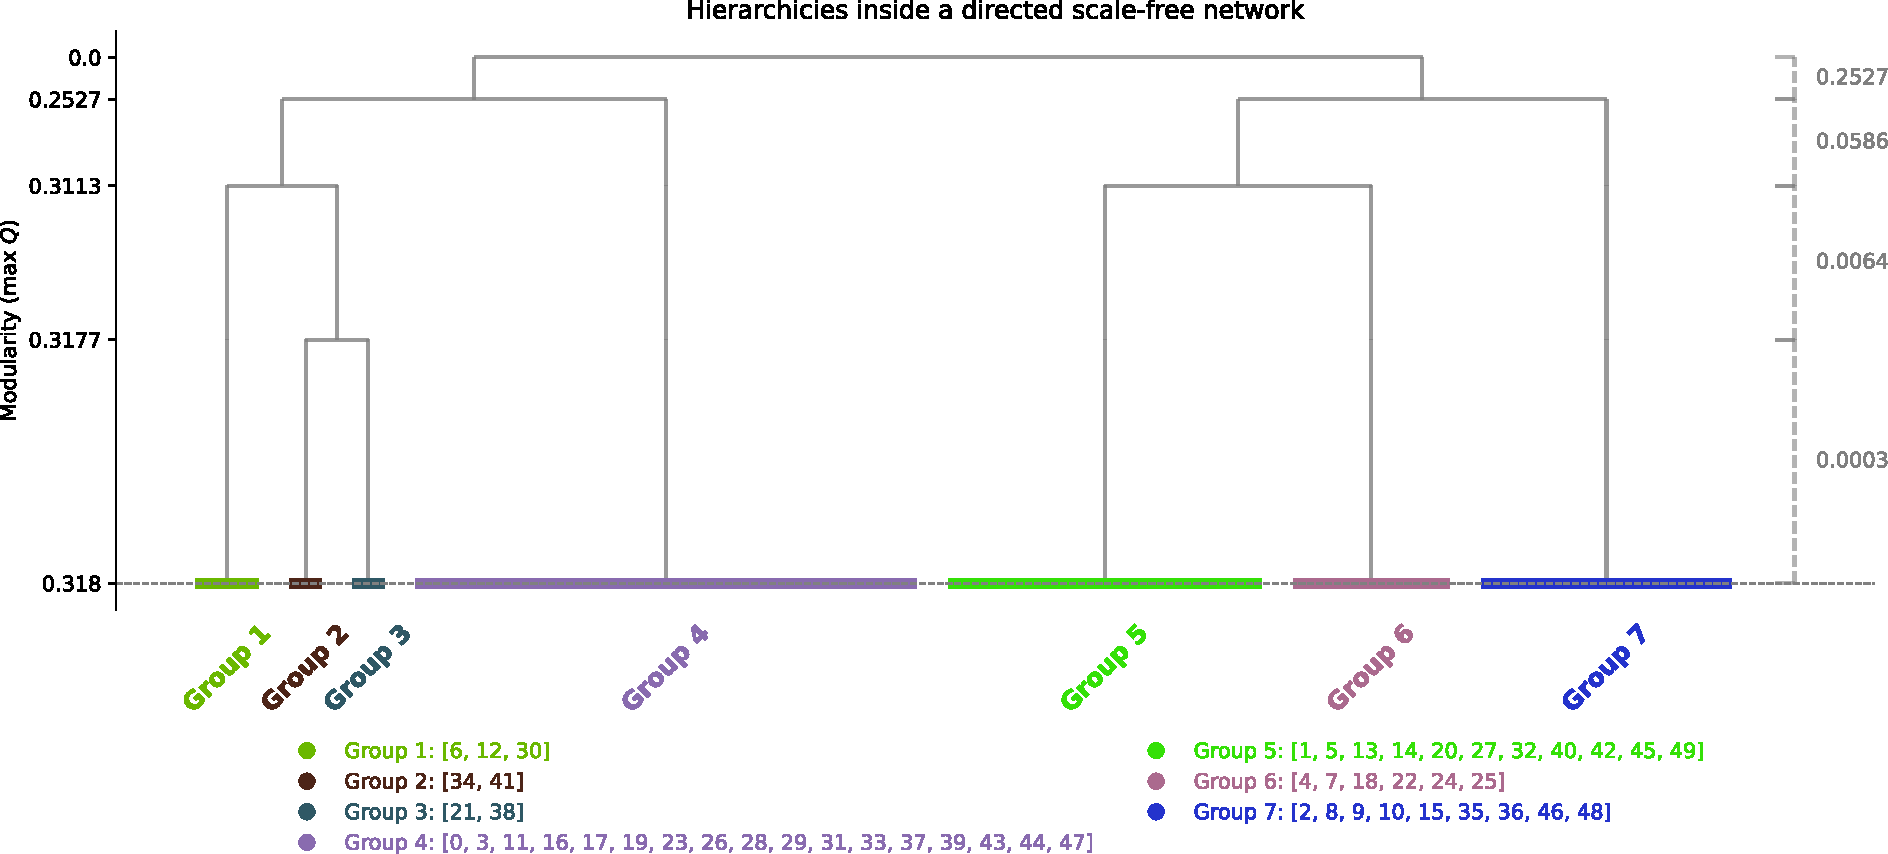
\includegraphics[width=1\linewidth]{Figures/FigS6.pdf}
    \caption{\textbf{Dendrogram of a directed sclae-free network \cite{bollobas2003} of N=50 nodes} Hierarchical structure found by the H. annealing algorithm. The hierarchy corresponds to the one unraveled after maximizing the modularity of the network as described in the main text; that is, {\tt num\_runs = 50} and {\tt resolution = 1}. Both the Louvain and Leiden algorithms returned a maximum modularity of $Q=0.31975$.}
    \label{fig:dendro_er}
\end{figure}

\begin{figure}[h]
    \centering
    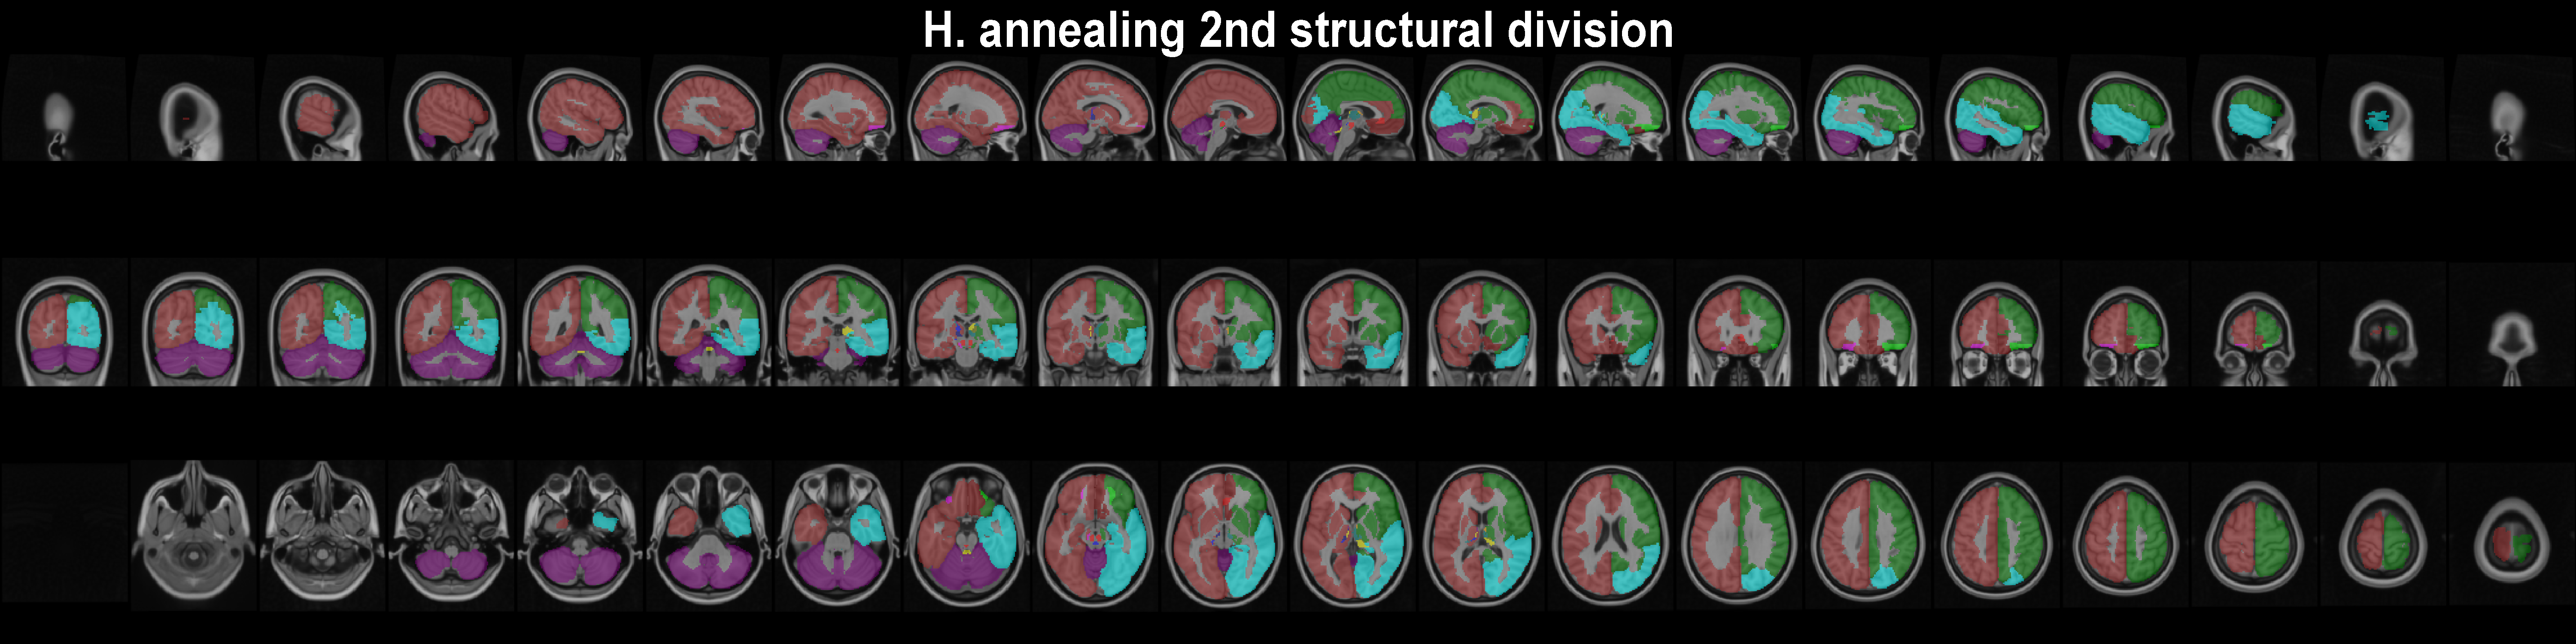
\includegraphics[width=1\linewidth]{Figures/FigS7.pdf}
    \caption{\textbf{Structural communities found at the early steps of the H. annealing process.} We plot the community structure discovered during the 2nd division of the hierarchical method described in the main text. It is visible how the hierarchy carries concise anatomical information, thus being a valid way to inspect hidden structures within complex networks through quantum annealing optimization.}
    \label{fig:hannealing_early_division}
\end{figure}

\begin{figure}[h]
    \centering
    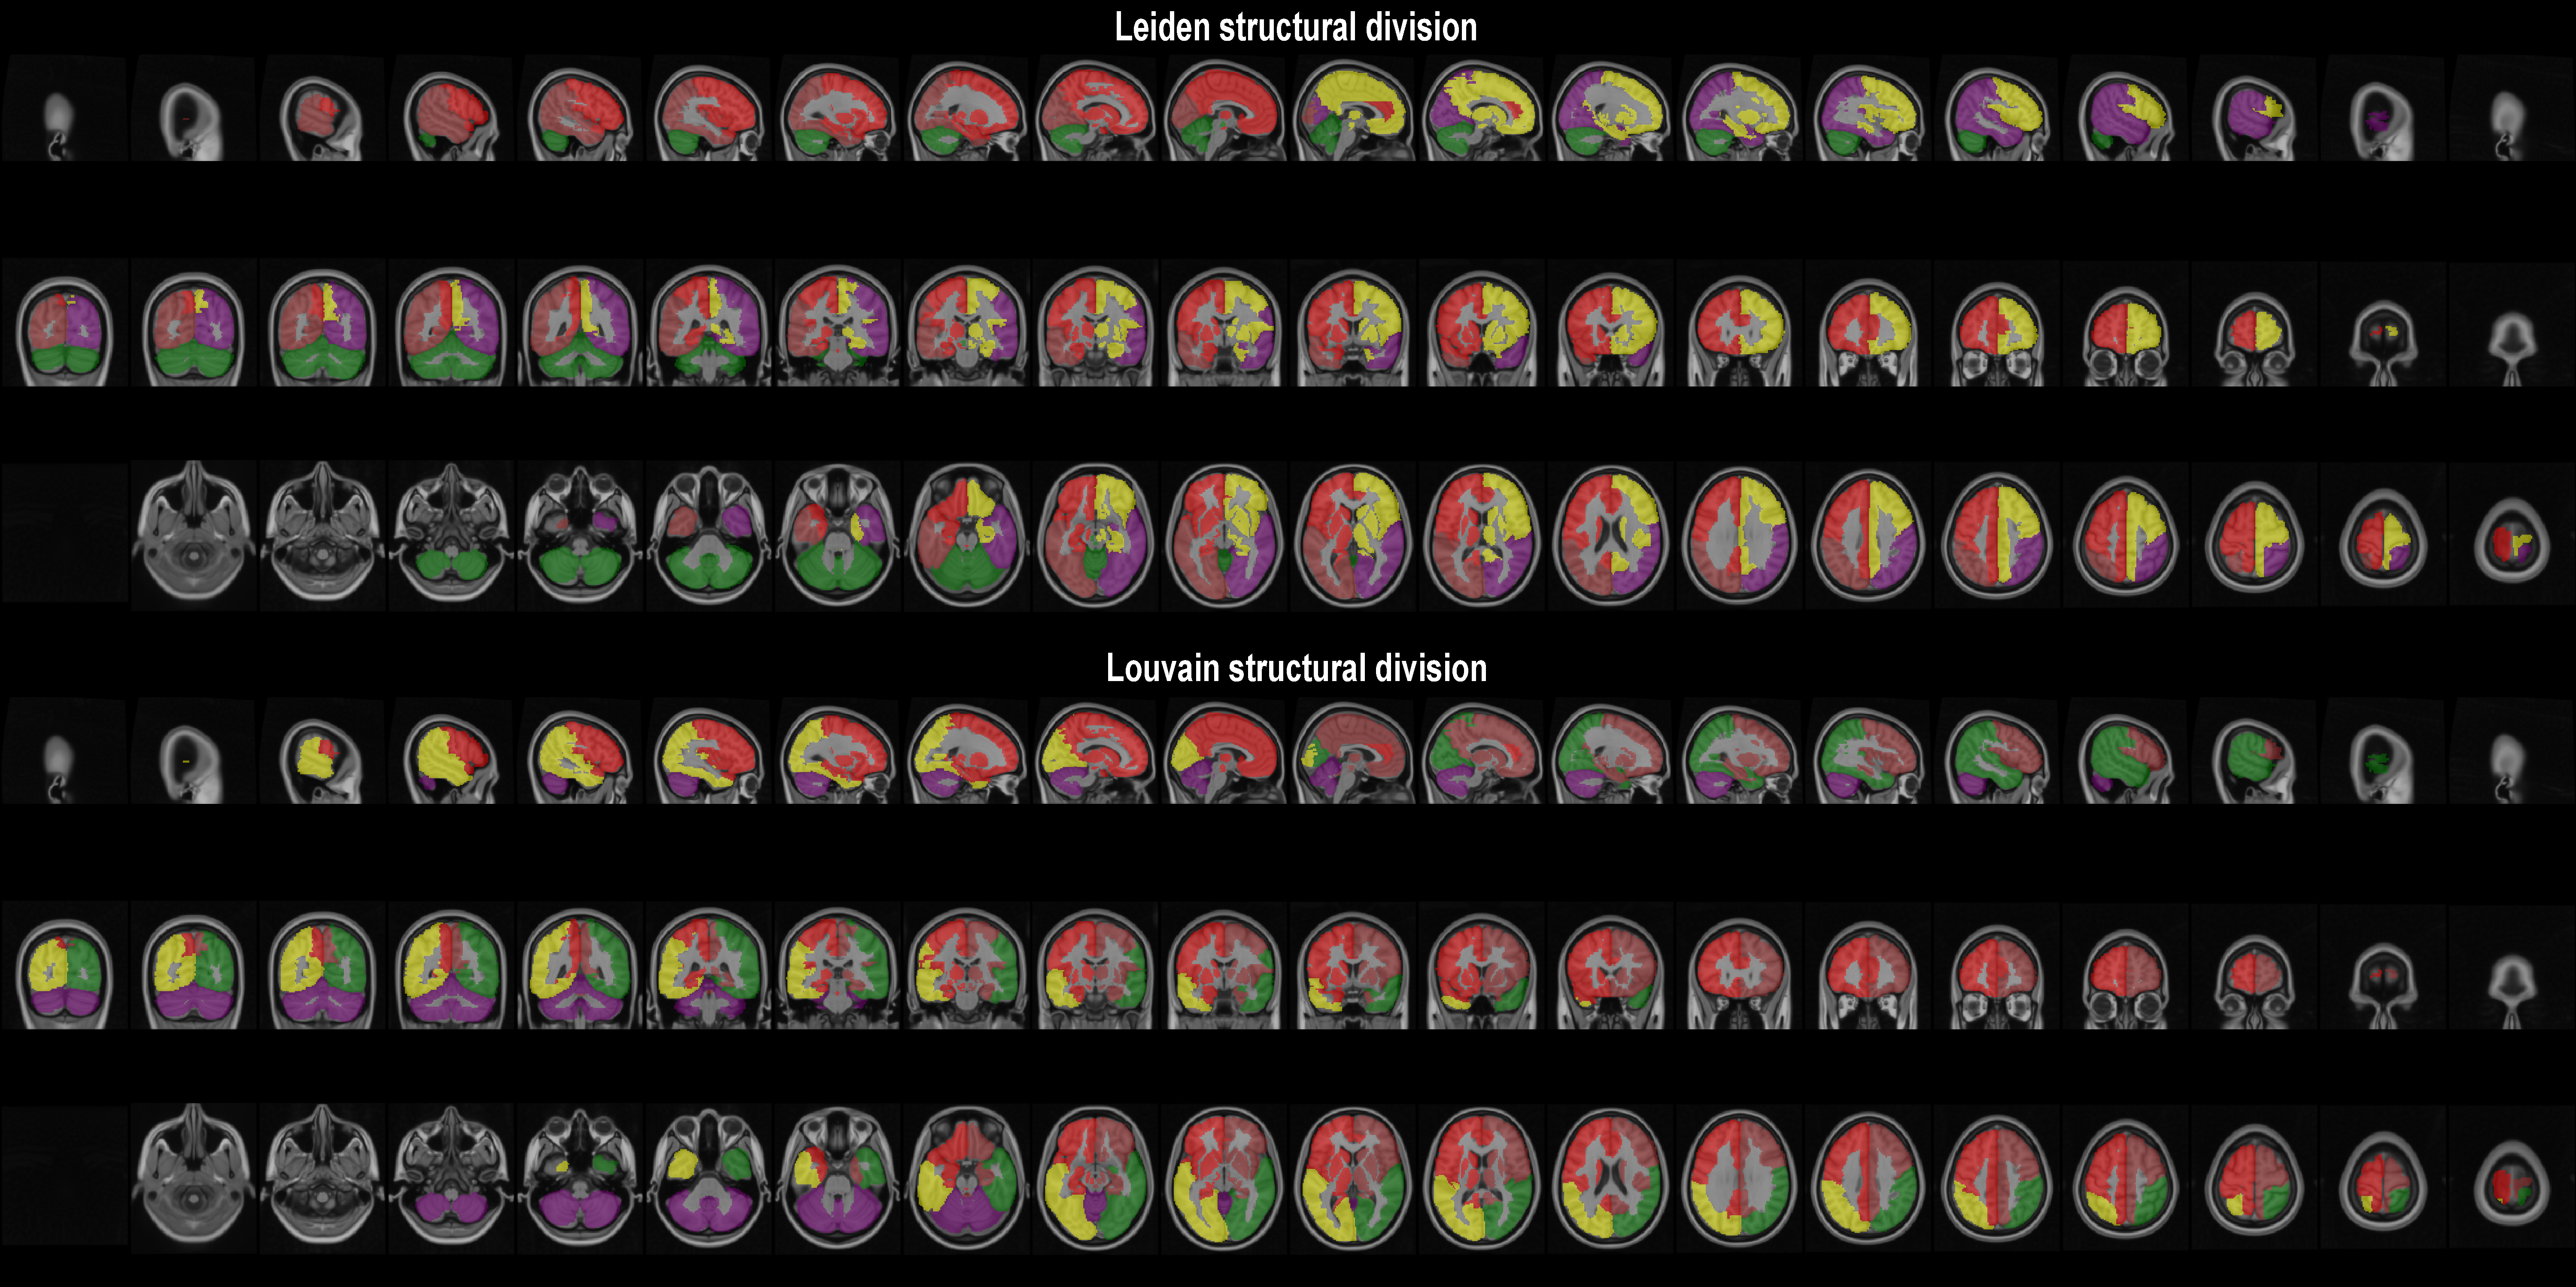
\includegraphics[width=1\linewidth]{Figures/FigS8.pdf}
    \caption{\textbf{Structural communities found by the Leiden and Louvain algorithms.} The resemblance between these communities and the ones found by the annealing process is strikingly high (see main text). The modularity found by the Leiden algorithm was $Q=0.610$, and the modularity returned by the Louvain algorithm was $Q=0.611$.}
    \label{fig:louva_leiden_structural}
\end{figure}

\clearpage
\section*{Software specifics: \textit{Qommunity}}

\subsection*{Architecture}
\begin{figure}[h]
    \centering
    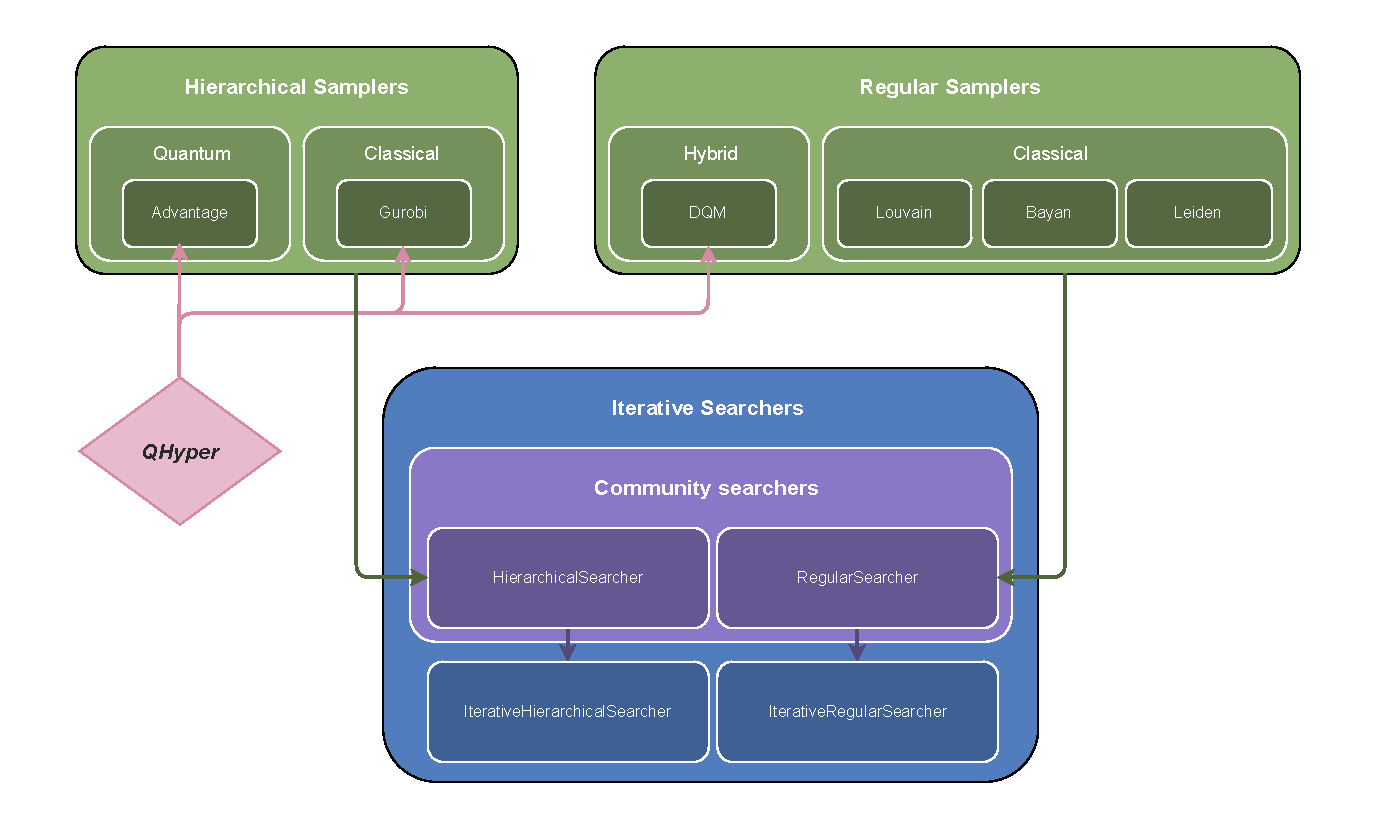
\includegraphics[width=1\linewidth]{Figures/FigS9.pdf}
    \caption{\textbf{Architecture of \textit{Qommunity} library}. The package makes use of the quantum computing library QHyper \cite{lamza_qhyper_2024} to communicate with the quantum annealer using multiple instances of a quadratic binary optimization problem. The Qommunity library also allows the user to choose from several other algorithms and solvers described in the main text. Lastly, the modularity maximization happens at the {\tt IterativeSearcher} class, where any solver and algorithm can be explicitly and automatically run an arbitrary number of times to produce a sufficiently big number of solutions to choose from.}
    \label{fig:qommunity_architecture}
\end{figure}

The \textit{Qommunity} library was designed to integrate several methods for detecting communities in graphs in one place. The implemented methods rely on classical, quantum, and hybrid solutions. The idea was to simplify and standardize the interface for conducting experiments. Several components compartmentalize the architecture, offering user-friendly features: Samplers, Searchers, and IterativeSearchers (Fig. \ref{fig:qommunity_architecture}).

\textit{\textbf{Samplers:}} Through Samplers we specify the method by which we want to detect communities, providing the necessary parameters. Currently, several classical solutions are implemented, such as Gurobi, Louvain \cite{Blondel2008}, Bayan\cite{aref2023}, Leiden \cite{Traag2019}, hybrid -- using DQM \cite{Wierzbinski2023}, and purely quantum -- using Advantage \cite{Johnson2011,lamza_qhyper_2024}. We divided samplers based on how the divisions are done;
\begin{itemize} 
\item regular: the dividing into communities is done according to the algorithms specified inside the Sampler.\item hierarchical: perform binary divisions using classical methods or quantum annealing, depending on the Sampler specified. If no division is optimal, the Sampler returns a single community. Alternatively, each binary division can be further continued in the course of recursion logic provided by the HierarchicalSearcher.
 %binary splits are done, that can be further continued in the course of recursion, if used with the help of a HierarchicalSearcher,
%\item \textcolor{blue}{hierarchical: perform binary splits and are capable of performing optional binary splits, i.e. split only in favour of an optimal solution. The splitting happens as a result of objective function opitimisation or in the course of sampling, depending on the algorithm specified inside the Sampler class},
\end{itemize}

Although Samplers provide community detection methods and can perform the community divisions themselves, the Seacher and IterativeSearcher are the dedicated tools for the user to perform the community detection process comprehensively. 
%To perform community detection with the appropriate Sampler, an instance of it needs to be passed to either the Searcher or the IterativeSearcher.

\textit{\textbf{Searchers:}} Searchers are responsible for executing community detection and for the appropriate postprocessing of its results.  There are two types of Searchers - hierarchical, which accept Samplers that perform hierarchical divisions of communities, and regular, which perform a non-hierarchical, regular community detection method. Each option is defined by the algorithm of choice 
%within the Sampler 
as follows: 
%However, the Searchers full scope of responsibility and action depends on their type:
\begin{itemize}
\item regular: they serve as wrappers for the RegularSampler, facilitating the regular community detection.
\item hierarchical: they extend the scope of action far beyond the RegularSearchers, by implementing the logic of recursion in the hierarchical search.  They build the construct of recursive calls. Its execution results in a tree of binary splits. Similar to RegularSearchers, they also wrap the appropriate Sampler, but with a different purpose - to call the community detection method on HierarchicalSampler on each recursion level and, depending on whether a binary split has occurred as its result, decide whether to proceed with recursion. Hence, they build and oversee the process of hierarchical community detection search, described in Algorithm 1 in the Main text.

The hierarchical searchers track the trace of the hierarchical divisions and, if specified by the user, can return it as a division tree, alongside division modularities, corresponding to each hierarchy division level.
\end{itemize}

\textit{\textbf{Iterative Searchers:}}  Iterative Searchers serve as wrappers for community Searchers, responsible for calling their corresponding (i.e. regular or hierarchical) community search method a given number of times. These multiple calls are useful due to the stochastic and probabilistic natures of the algorithms \textit{Qommunity} provides.
As a result, for each iteration, we get a graph divided into communities, its modularity measure, and the execution time. The result may also contain the division trees and the division modularities, in the case of hierarchical community search. Iterative Searchers are used to simplify the execution of experiments aimed at maximizing the modularity of a given network (see Algorithm 2 in the Main text).

\subsection*{High-level Python code examples to use the quantum resources for modularity maximization and interpretation}
\begin{lstlisting}[language=Python, caption=Modularity maximization and community detection using \textit{Qommunity}. After importing the relevant Python modules maximizing the modularity of the network using quantum computing would be trivial., label=python1]
import networkx as nx # Hagberg, et al. 2008
import numpy as np

## ORIGINAL FROM THIS WORK
from Qommunity.samplers.hierarchical.advantage_sampler import AdvantageSampler # H. Annealing
from Qommunity.samplers.hierarchical.gurobi_sampler import GurobiSampler # H. Gurobi

## HYBRID QUANTUM SOLVER (Wierzbinski, et al. 2023)
from Qommunity.samplers.regular.dqm_sampler import DQMSampler 

## ALETERNATIVE BENCHAMRKS
from Qommunity.samplers.regular.bayan_sampler import BayanSampler 
from Qommunity.samplers.regular.leiden_sampler import LeidenSampler
from Qommunity.samplers.regular.louvain_sampler import LouvainSampler

## MODULARITY MAXIMIZATION
from iterative_searcher.iterative_searcher import IterativeSearcher

## NETWORK TO ANALYZE
Graph = nx.karate_club_graph()
# Graph = nx.from_numpy_array(np.genfromtxt("A.csv", delimiter=','))

## PARAMETERS
num_runs = 20
resolution = 1 #

## Initiate the quantum processor and generate the QUBO
adv_sampler = AdvantageSampler(
    Graph, 
    resolution=resolution, 
    num_reads=100, 
    use_clique_embedding=True
)
adv_iterative= IterativeSearcher(adv_sampler)
communities, modularities, times = adv_iterative.run(num_runs=num_runs, save_results=False)

# Only the community with the highest modularity
community_structure = communities[modularities.argmax()]
modularity = modularities.max()
elapsed_time = times[modularities.argmax()]

\end{lstlisting}

\begin{lstlisting}[language=Python, caption=Example to obtain the hierarchical structure of a given network using modularity maximization., label=python2]
import networkx as nx
import numpy as np
import matplotlib.pylab as plt

## IMPORT THE RELEVANT MODULES
from Qommunity.samplers.hierarchical.advantage_sampler import AdvantageSampler
from iterative_searcher.iterative_searcher import IterativeSearcher
from dendro import Dendrogram

## PARAMETERS
num_runs = 20
resolution = 1

## NETWORK
G = nx.karate_club_graph()
# Graph = nx.from_numpy_array(np.genfromtxt("A.csv", delimiter=','))

# COMMUNITY DETECTION USING RECUSRIVE QUANTUM ANNEALING
searcher = IterativeSearcher(
    AdvantageSampler(
        G, 
        resolution=resolution, 
        num_reads=100, 
        use_clique_embedding=True
    )
)
results = searcher.run_with_sampleset_info(num_runs=num_runs, save_results=False, saving_path=None, iterative_verbosity=0)

## MODULARITY MAXIMIZATION (Algorithm 2 in the main Methods)
mods_Adv = results.modularity
communities = results.communities[mods_Adv.argmax()]
division_tree = results.division_tree[mods_Adv.argmax()]
division_modularities = results.division_modularities[mods_Adv.argmax()]
time = results.time[mods_Adv.argmax()]

## PLOTTING AND CUSTOMIZING THE HIERARCHY PLOT
dendro = Dendrogram(G, communities, division_modularities, division_tree)
fig, ax = plt.subplots(1,1,figsize=(13,6))
dendro.draw(
    display_leafs=False,
    yaxis_abs_log=True,
    ax=ax,
    fig=fig,
    communities_labels=["Group 1", "Group 2", "Group 3", "Group 4", "Group 5", "Group 6", "Group 7", "Group 8"],
    fig_saving_path="./Karate/dendrogram.svg",
    title='Hierarchicies inside the Karate network'
)
\end{lstlisting}

\bibliography{main}% common bib file
%% if required, the content of .bbl file can be included here once bbl is generated
%%\input sn-article.bbl

\end{document}